% !TeX spellcheck = da_DK
\subsection{Filtrering}
Filtrering er et værktøj indenfor databehandling, som anvendes i det biologiske signals frekvensdomæne. Formålet med at filtrere et målt signal er at fjerne uønskede frekvenser, også kaldet støj, der ikke tilhører det signal, der ønskes undersøgt. Filtret kan opdele signalet i såkaldte bånd: Pasbånd, hvor frekvenserne frit passerer igennem filteret uden påvirkning, samt stopbånd, hvor frekvenserne dæmpes, så de ikke har indflydelse på signalet. Dette gøres ved en knækfrekvens.
Der findes flere forskellige typer af filtre, der afhænger af, hvilke frekvenser der skal fjernes fra det målte signal \cite{Devasahayam2000}:

\begin{itemize}
	\item Lavpasfiltret: Anvendes til at dæmpe frekvenser over den valgte knækfrekvens. Dette gøres ved at dæmpe de frekvenser, som ligger over knækfrekvensen.
	\item Højpasfilteret: Anvendes, modsat lavpasfiltret, til at dæmpe frekvenser under den valgte knækfrekvens ved at dæmpe signalet under knækfrekvensen.
	\item Båndpasfilteret: Er en kombination af et lav- og højpasfilter.  Her defineres et interval, hvormed de frekvenser der ligger udenfor intervallet vil blive dæmpet.
	\item Båndstopfilteret: Fungerer, modsat båndpasfilteret, ved at dæmpe specifikt definerede frekvensområder. Frekvenserne udenfor det definerede område påvirkes ikke. 
\end{itemize}
  
I forbindelse med databehandling kan flere af filtrene anvendes samtidig \cite{Devasahayam2000}. Princippet i de fire filtertyper er illustreret på \figref{filtertyper}.
\begin{figure}[H]
\centering
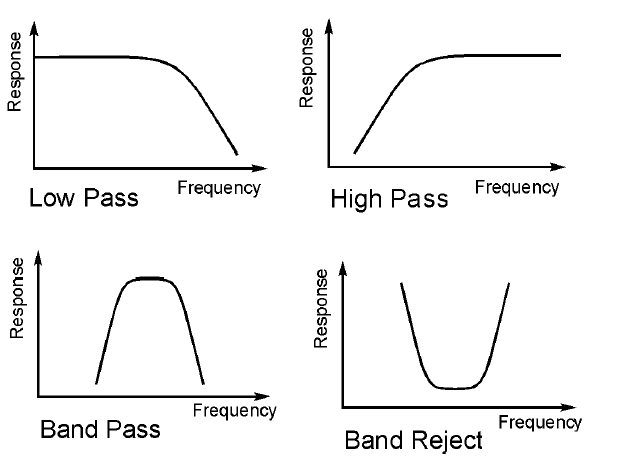
\includegraphics[scale=0.8]{figures/bproblemanalyse/filtertyper.png}
\caption{De fire filtertyper ses her \cite{2. semester kristian}\fxnote{Må man citere til en forelæsning?}}
\label{filtertyper}
\end{figure}
Filtrene kan desuden inddeles i forskellige grader eller ordener, afhængigt af hvor stejl filtreringskurven er, dvs. hvor meget signalet dæmpes pr. dekade\cite{2. semester kristian}.

\subsection{Støj}
Støj er den uønskede del af et opsamlet signal, der ikke har nogen relation til det ønskede signal \fxnote{Må man citere til en forelæsning? - Hvis ja, så ved Nikoline, hvilken forelæsning det er}. Signaler, der er fordelt udover et frekvensspektrum, kan filtreres for støj vha. de tidligere beskrevne filtre. \cite{Devasahayam2000}
Støj kan inddeles i flere forskellige generelle typer, som typisk vil forekomme:

\begin{itemize}
\item Elektriske signaler: Dette er bl.a. 50 Hz støj, som er en frekvens fra elnettet. Denne 50 Hz frekvens kan gå ind og påvirke de biologiske signaler, der måles på. Hvis der er flere 50 Hz kilder, der interagerer, kan det give ekko ved eksempelvis 100 Hz og 150 Hz. Det er denne form for støj, der skal undgås, når signalet analyseres.
\item Ledninger: Kan fungere som antenner, der opfanger 50 Hz støj og andre former for støj. Problemet bliver større jo længere ledningen er. 
\item Magnetfelt: Kan komme i kontakt med ledningerne og derved inducere strømmen, der skaber støj i signalet. Jordens magnetfelt kan f.eks. påvirke ledningerne. For at mindske støjen kan ledningerne snoes / flettes sammen.
\end{itemize} 